
%(BEGIN_QUESTION)
% Copyright 2011, Tony R. Kuphaldt, released under the Creative Commons Attribution License (v 1.0)
% This means you may do almost anything with this work of mine, so long as you give me proper credit

Examine the ``Siemens/Moore 353 program for pulse-width modulation'' contained on your Instrumentation Reference, showing a function block program for equipping the 353 controller with a PWM output signal (modulated on/off) rather than an analog 4-20 mA output signal, then answer the following questions:

\vskip 10pt

Identify those function blocks which are connected identically to the standard Factory Configured Option 101 program, then identify those function blocks which are different.

\vskip 10pt

Explain why anyone would wish to have a loop controller equipped with a PWM output instead of a 4-20 mA analog output.

\vskip 10pt

Explain how this analog circuit functions to produce a PWM output signal from a sawtooth waveform and a DC reference signal, and how this functionality is mimicked by the function block program of the Siemens 353 controller:

$$\includegraphics[width=15.5cm]{i00356x01.eps}$$



\vskip 20pt \vbox{\hrule \hbox{\strut \vrule{} {\bf Suggestions for Socratic discussion} \vrule} \hrule}

\begin{itemize}
\item{} Describe the steps necessary to edit the FCO 101 program so that it resembles this program, using the faceplate pushbutton controls and displays.
\item{} Which way would you have to move the wiper on the potentiometer in the analog circuit in order to increase the duty cycle of the PWM output?
\item{} What would be the effect of the +V power source connection to the potentiometer failing open?
\item{} What would be the effect of the ground connection to the potentiometer failing open?
\item{} What would be the effect of the sawtooth wave generator connection failing with a 0 volt output?
\item{} What would be the effect of the +V power source connection to the comparator failing open?
\item{} Sketch the diagram of an ``interposing'' circuit that can take the opamp's output signal and amplify it to drive PWM power to a large electric heating element (e.g. rated at a much greater voltage such as 240 VAC).
\end{itemize}

\underbar{file i00356}
%(END_QUESTION)





%(BEGIN_ANSWER)


%(END_ANSWER)





%(BEGIN_NOTES)

The AIN1, SETPT, PID, and A/M function blocks are all part of the stock FCO 101 program.  All the other blocks have been added to make this particular PWM function.

\vskip 10pt

A controller program with a PWM output would be useful if the controller were driving a discrete FCO such as an electrical heating element (on/off) or a solenoid valve.

\vskip 10pt

The comparator compares the sawtooth voltage signal against the DC reference set by the potentiometer.  Whenever the DC reference voltage exceeds the sawtooth voltage, the output of the comparator goes high.  As the sawtooth voltage signal rises and falls, the comparator output switches between high and low states, creating a pulse wave signal.  As the DC reference voltage is increased, the time spent in the ``high'' state will be longer and the time spent in the ``low'' state will be shorter, thereby increasing the pulse signal's duty cycle.

%INDEX% Reading assignment: Siemens model 353 controller program for PWM control

%(END_NOTES)


